\documentclass{standalone}
\usepackage{tikz}
\usetikzlibrary{patterns, positioning}

\begin{document}
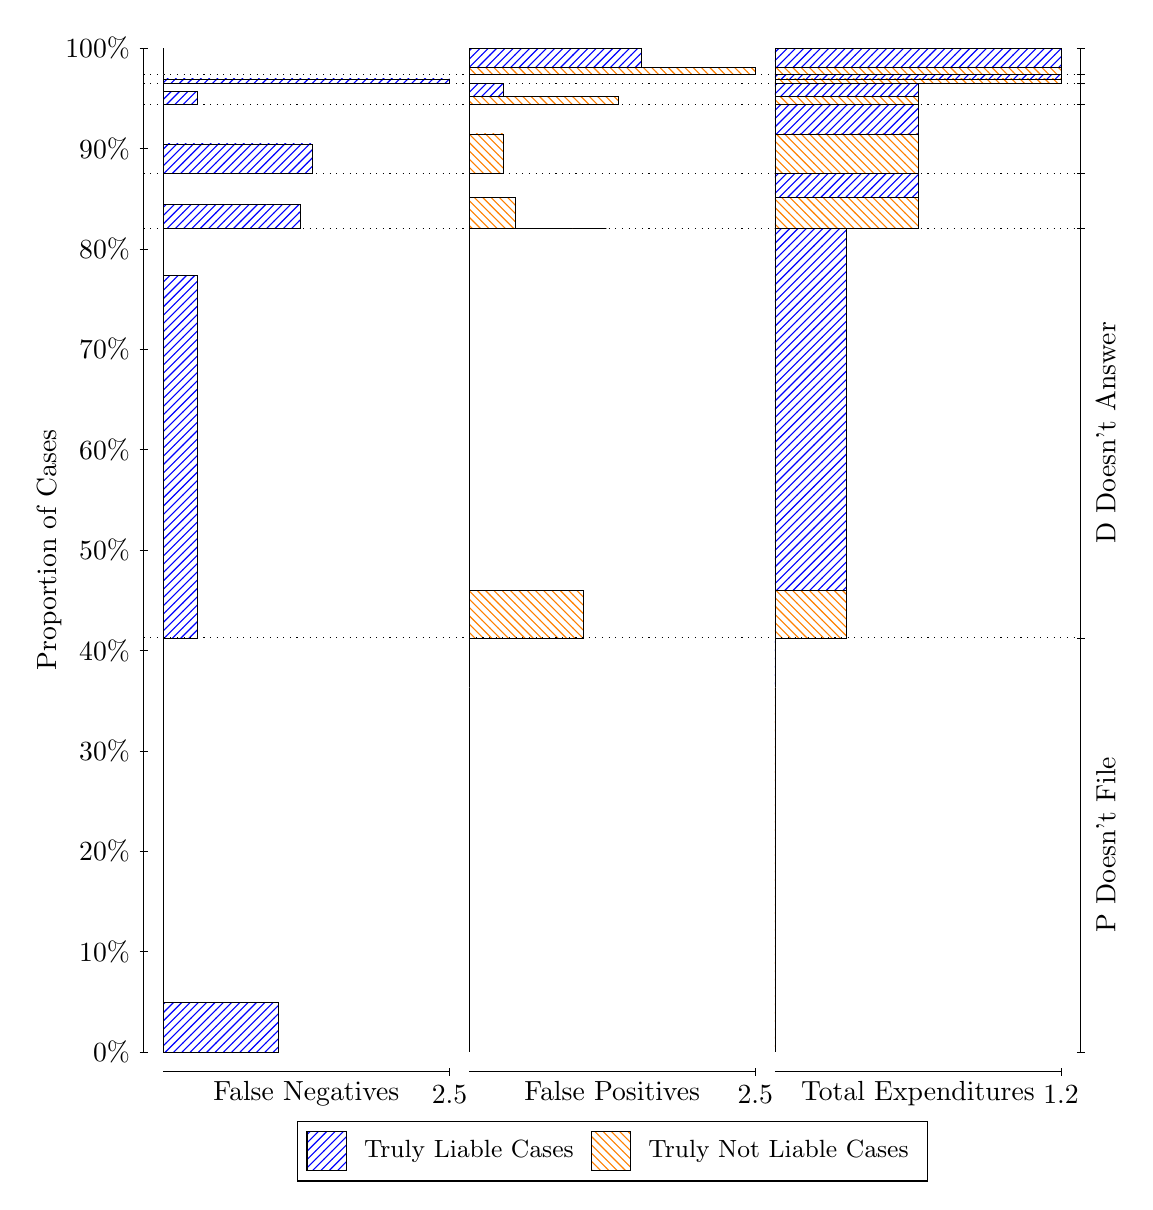
\begin{tikzpicture}
\draw[black, very thin] (1.5,1.75) -- (1.5,14.5);
\node[rotate=90, anchor=center] at (0.3, 8.125) {Proportion of Cases};
\draw[black, very thin] (1.45,1.75) -- (1.55,1.75);
\node[anchor=east] at (1.45, 1.75) {0\%};
\draw[black, very thin] (1.45,3.025) -- (1.55,3.025);
\node[anchor=east] at (1.45, 3.025) {10\%};
\draw[black, very thin] (1.45,4.3) -- (1.55,4.3);
\node[anchor=east] at (1.45, 4.3) {20\%};
\draw[black, very thin] (1.45,5.575) -- (1.55,5.575);
\node[anchor=east] at (1.45, 5.575) {30\%};
\draw[black, very thin] (1.45,6.85) -- (1.55,6.85);
\node[anchor=east] at (1.45, 6.85) {40\%};
\draw[black, very thin] (1.45,8.125) -- (1.55,8.125);
\node[anchor=east] at (1.45, 8.125) {50\%};
\draw[black, very thin] (1.45,9.4) -- (1.55,9.4);
\node[anchor=east] at (1.45, 9.4) {60\%};
\draw[black, very thin] (1.45,10.675) -- (1.55,10.675);
\node[anchor=east] at (1.45, 10.675) {70\%};
\draw[black, very thin] (1.45,11.95) -- (1.55,11.95);
\node[anchor=east] at (1.45, 11.95) {80\%};
\draw[black, very thin] (1.45,13.225) -- (1.55,13.225);
\node[anchor=east] at (1.45, 13.225) {90\%};
\draw[black, very thin] (1.45,14.5) -- (1.55,14.5);
\node[anchor=east] at (1.45, 14.5) {100\%};

\draw[black, very thin] (13.4,1.75) -- (13.4,14.5);
\draw[black, very thin] (13.35,1.75) -- (13.45,1.75);
\node[anchor=west] at (13.35, 1.75) {};
\draw[black, very thin] (13.35,7.01) -- (13.45,7.01);
\node[anchor=west] at (13.35, 7.01) {};
\draw[black, very thin] (13.35,12.211) -- (13.45,12.211);
\node[anchor=west] at (13.35, 12.211) {};
\draw[black, very thin] (13.35,12.909) -- (13.45,12.909);
\node[anchor=west] at (13.35, 12.909) {};
\draw[black, very thin] (13.35,13.786) -- (13.45,13.786);
\node[anchor=west] at (13.35, 13.786) {};
\draw[black, very thin] (13.35,14.05) -- (13.45,14.05);
\node[anchor=west] at (13.35, 14.05) {};
\draw[black, very thin] (13.35,14.166) -- (13.45,14.166);
\node[anchor=west] at (13.35, 14.166) {};
\draw[black, very thin] (13.35,14.5) -- (13.45,14.5);
\node[anchor=west] at (13.35, 14.5) {};

\draw[black, very thin, pattern color=blue, pattern=north east lines] (1.75,1.75) rectangle (3.2033,2.3828);
\draw[black, very thin, pattern color=orange, pattern=north west lines] (1.75,2.3828) rectangle (1.75,7.01);
\draw[black, very thin, pattern color=blue, pattern=north east lines] (1.75,7.01) rectangle (2.186,11.608);
\draw[black, very thin, pattern color=orange, pattern=north west lines] (1.75,11.608) rectangle (1.75,12.211);
\draw[black, very thin, pattern color=blue, pattern=north east lines] (1.75,12.211) rectangle (3.494,12.515);
\draw[black, very thin, pattern color=blue, pattern=north east lines] (1.75,12.515) rectangle (3.3487,12.515);
\draw[black, very thin, pattern color=blue, pattern=north east lines] (1.75,12.515) rectangle (3.2033,12.515);
\draw[black, very thin, pattern color=blue, pattern=north east lines] (1.75,12.515) rectangle (3.058,12.515);
\draw[black, very thin, pattern color=blue, pattern=north east lines] (1.75,12.515) rectangle (3.058,12.515);
\draw[black, very thin, pattern color=blue, pattern=north east lines] (1.75,12.515) rectangle (2.9127,12.515);
\draw[black, very thin, pattern color=blue, pattern=north east lines] (1.75,12.515) rectangle (2.7673,12.515);
\draw[black, very thin, pattern color=blue, pattern=north east lines] (1.75,12.515) rectangle (2.622,12.515);
\draw[black, very thin, pattern color=blue, pattern=north east lines] (1.75,12.515) rectangle (2.4767,12.515);
\draw[black, very thin, pattern color=blue, pattern=north east lines] (1.75,12.515) rectangle (2.3313,12.515);
\draw[black, very thin, pattern color=orange, pattern=north west lines] (1.75,12.515) rectangle (1.75,12.909);
\draw[black, very thin, pattern color=blue, pattern=north east lines] (1.75,12.909) rectangle (3.6393,13.284);
\draw[black, very thin, pattern color=orange, pattern=north west lines] (1.75,13.284) rectangle (1.75,13.786);
\draw[black, very thin, pattern color=blue, pattern=north east lines] (1.75,13.786) rectangle (2.186,13.951);
\draw[black, very thin, pattern color=orange, pattern=north west lines] (1.75,13.951) rectangle (1.75,14.05);
\draw[black, very thin, pattern color=blue, pattern=north east lines] (1.75,14.05) rectangle (5.3833,14.109);
\draw[black, very thin, pattern color=orange, pattern=north west lines] (1.75,14.109) rectangle (1.75,14.166);
\draw[black, very thin, pattern color=orange, pattern=north west lines] (1.75,14.166) rectangle (1.75,14.258);
\draw[black, very thin, pattern color=blue, pattern=north east lines] (1.75,14.258) rectangle (1.75,14.5);
\draw[black, very thin, pattern color=orange, pattern=north west lines] (5.6333,1.75) rectangle (5.6333,6.3773);
\draw[black, very thin, pattern color=blue, pattern=north east lines] (5.6333,6.3773) rectangle (5.6333,7.01);
\draw[black, very thin, pattern color=orange, pattern=north west lines] (5.6333,7.01) rectangle (7.0867,7.6132);
\draw[black, very thin, pattern color=blue, pattern=north east lines] (5.6333,7.6132) rectangle (5.6333,12.211);
\draw[black, very thin, pattern color=orange, pattern=north west lines] (5.6333,12.211) rectangle (7.3773,12.211);
\draw[black, very thin, pattern color=orange, pattern=north west lines] (5.6333,12.211) rectangle (7.232,12.211);
\draw[black, very thin, pattern color=orange, pattern=north west lines] (5.6333,12.211) rectangle (7.0867,12.211);
\draw[black, very thin, pattern color=orange, pattern=north west lines] (5.6333,12.211) rectangle (6.9413,12.211);
\draw[black, very thin, pattern color=orange, pattern=north west lines] (5.6333,12.211) rectangle (6.796,12.211);
\draw[black, very thin, pattern color=orange, pattern=north west lines] (5.6333,12.211) rectangle (6.6507,12.211);
\draw[black, very thin, pattern color=orange, pattern=north west lines] (5.6333,12.211) rectangle (6.5053,12.211);
\draw[black, very thin, pattern color=orange, pattern=north west lines] (5.6333,12.211) rectangle (6.36,12.211);
\draw[black, very thin, pattern color=orange, pattern=north west lines] (5.6333,12.211) rectangle (6.2147,12.605);
\draw[black, very thin, pattern color=blue, pattern=north east lines] (5.6333,12.605) rectangle (5.924,12.605);
\draw[black, very thin, pattern color=blue, pattern=north east lines] (5.6333,12.605) rectangle (5.7787,12.605);
\draw[black, very thin, pattern color=blue, pattern=north east lines] (5.6333,12.605) rectangle (5.6333,12.909);
\draw[black, very thin, pattern color=orange, pattern=north west lines] (5.6333,12.909) rectangle (6.0693,13.41);
\draw[black, very thin, pattern color=blue, pattern=north east lines] (5.6333,13.41) rectangle (5.6333,13.786);
\draw[black, very thin, pattern color=orange, pattern=north west lines] (5.6333,13.786) rectangle (7.5227,13.886);
\draw[black, very thin, pattern color=blue, pattern=north east lines] (5.6333,13.886) rectangle (6.0693,14.05);
\draw[black, very thin, pattern color=orange, pattern=north west lines] (5.6333,14.05) rectangle (5.6333,14.108);
\draw[black, very thin, pattern color=blue, pattern=north east lines] (5.6333,14.108) rectangle (5.6333,14.166);
\draw[black, very thin, pattern color=orange, pattern=north west lines] (5.6333,14.166) rectangle (9.2667,14.258);
\draw[black, very thin, pattern color=blue, pattern=north east lines] (5.6333,14.258) rectangle (7.8133,14.5);
\draw[black, very thin, pattern color=orange, pattern=north west lines] (9.5167,1.75) rectangle (9.5167,6.3773);
\draw[black, very thin, pattern color=blue, pattern=north east lines] (9.5167,6.3773) rectangle (9.5167,7.01);
\draw[black, very thin, pattern color=orange, pattern=north west lines] (9.5167,7.01) rectangle (10.425,7.6132);
\draw[black, very thin, pattern color=blue, pattern=north east lines] (9.5167,7.6132) rectangle (10.425,12.211);
\draw[black, very thin, pattern color=orange, pattern=north west lines] (9.5167,12.211) rectangle (11.333,12.211);
\draw[black, very thin, pattern color=blue, pattern=north east lines] (9.5167,12.211) rectangle (11.333,12.211);
\draw[black, very thin, pattern color=orange, pattern=north west lines] (9.5167,12.211) rectangle (11.333,12.605);
\draw[black, very thin, pattern color=blue, pattern=north east lines] (9.5167,12.605) rectangle (11.333,12.909);
\draw[black, very thin, pattern color=orange, pattern=north west lines] (9.5167,12.909) rectangle (11.333,12.909);
\draw[black, very thin, pattern color=blue, pattern=north east lines] (9.5167,12.909) rectangle (11.333,12.909);
\draw[black, very thin, pattern color=orange, pattern=north west lines] (9.5167,12.909) rectangle (11.333,13.41);
\draw[black, very thin, pattern color=blue, pattern=north east lines] (9.5167,13.41) rectangle (11.333,13.786);
\draw[black, very thin, pattern color=orange, pattern=north west lines] (9.5167,13.786) rectangle (11.333,13.886);
\draw[black, very thin, pattern color=blue, pattern=north east lines] (9.5167,13.886) rectangle (11.333,14.05);
\draw[black, very thin, pattern color=orange, pattern=north west lines] (9.5167,14.05) rectangle (13.15,14.108);
\draw[black, very thin, pattern color=blue, pattern=north east lines] (9.5167,14.108) rectangle (13.15,14.166);
\draw[black, very thin, pattern color=orange, pattern=north west lines] (9.5167,14.166) rectangle (13.15,14.258);
\draw[black, very thin, pattern color=blue, pattern=north east lines] (9.5167,14.258) rectangle (13.15,14.5);
\draw[black, dotted] (1.5,7.01) -- (13.4,7.01);
\draw[black, dotted] (1.5,12.211) -- (13.4,12.211);
\draw[black, dotted] (1.5,12.909) -- (13.4,12.909);
\draw[black, dotted] (1.5,13.786) -- (13.4,13.786);
\draw[black, dotted] (1.5,14.05) -- (13.4,14.05);
\draw[black, dotted] (1.5,14.166) -- (13.4,14.166);
\draw[black, very thin] (1.75,1.5) -- (5.3833,1.5);
\node[anchor=north] at (3.5667, 1.5) {False Negatives};
\draw[black, very thin] (5.3833,1.45) -- (5.3833,1.55);
\node[anchor=north] at (5.3833, 1.45) {2.5};

\draw[black, very thin] (5.6333,1.5) -- (9.2667,1.5);
\node[anchor=north] at (7.45, 1.5) {False Positives};
\draw[black, very thin] (9.2667,1.45) -- (9.2667,1.55);
\node[anchor=north] at (9.2667, 1.45) {2.5};

\draw[black, very thin] (9.5167,1.5) -- (13.15,1.5);
\node[anchor=north] at (11.333, 1.5) {Total Expenditures};
\draw[black, very thin] (13.15,1.45) -- (13.15,1.55);
\node[anchor=north] at (13.15, 1.45) {1.2};

\node[black, centered, rotate=90] at (13.72, 4.38) {P Doesn't File};
\node[black, centered, rotate=90] at (13.72, 9.6105) {D Doesn't Answer};






\draw (7.449999999999999,1.5) node[draw=none] (baseCoordinate) {};
\begin{scope}[align=center]
        \matrix[scale=0.5, draw=black, below=0.5cm of baseCoordinate, nodes={draw}, column sep=0.1cm]{
            \node[rectangle, draw, minimum width=0.5cm, minimum height=0.5cm, pattern=north east lines, pattern color=blue] {}; &
            \node[draw=none, font=\small] (B) {Truly Liable Cases}; &
            \node[rectangle, draw, minimum width=0.5cm, minimum height=0.5cm, pattern=north west lines, pattern color=orange] {}; &
            \node[draw=none, font=\small] (B) {Truly Not Liable Cases}; \\
            };
\end{scope}

\end{tikzpicture}
\end{document}